\section{Physics beyond the Standard Model}
\label{sec:bsm}

For a long time the completion of the \sm was reliant on the discovery of the Higgs boson.
Finally, in 2012, the \cms~\cite{Chatrchyan:2008aa} and \atlas~\cite{Aad:2008zzm} collaborations
observed a Higgs-like boson with a mass of $m_H\simeq125\gev$~\cite{Chatrchyan:2012ufa,Aad:2012tfa}.
This final piece of the picture has made the \sm a remarkably robust theory with no predictions
deviating significantly from experimental observations.
Indeed, the theory of \QED~--- which describes interactions between
photons and charged particles in the \sm --- is one of the most accurate theories yet constructed.
The coupling constant in \QED is the fine structure constant, $\alpha$, which has been measured
experimentally to be~\cite{PDG2012}
\begin{align}
  \alpha^{-1}_\mathrm{exp} &= 137.035\,999\,074\,(44), \nonumber\\
  \intertext{and predicted theoretically to be~\cite{Aoyama:2012wj}}
  \alpha^{-1}_\mathrm{th} &= 137.035\,999\,073\,(35). \nonumber
\end{align}
These measurements have precisions which are better than one part per billion, and the extent to
which they agree is testament to our understanding of \QED interactions.
%\begin{align}
  %\phantom{.} &&\alpha^{-1}_\mathrm{exp} &= 137.035\,999\,074\,(44), && \text{\cite{PDG2012}} \nonumber\\
  %\intertext{cats are the best}
  %\phantom{.} &&\alpha^{-1}_\mathrm{th} &= 137.035\,999\,073\,(35), && \text{\cite{Aoyama:2012wj}}
%\end{align}

Despite its countless successes, there are a plethora of indications --- both
experimental and theoretical --- that additional physics exists, \bsm.


\subsection{Failures and inconsistencies of the Standard Model}
\label{sec:bsm:fail}
%%%%%%%%%%%%%%%%%%%%%%%%%%%%%%%%%%%%%%%%%%%%%%%%%%%%%%%%%%%%%%%%%%%%%%%%%%%%%%%%%%%%%%%%%%%%%%%%%%%
% Experimental
%%%%%%%%%%%%%%%%%%%%%%%%%%%%%%%%%%%%%%%%%%%%%%%%%%%%%%%%%%%%%%%%%%%%%%%%%%%%%%%%%%%%%%%%%%%%%%%%%%%
There are some phenomena that have been observed experimentally which cannot be explained by the
\sm.
Oscillations of neutrinos in flavour space mean that they must have mass; this is not accounted for
the \sm framework.
Neither are the observations of the \BAU, or \dm.

% CPV
The \sm cannot reconcile the matter-antimatter asymmetry observed in the
Universe today.
The hypothesized process which caused this asymmetry is known as baryogenesis.
Whatever this process may be it must satisfy the three Sakharov
conditions~\cite{1991SvPhU..34..392S}, which outline the minimum requirements for baryogenesis.
The first, most obvious, criteria is that baryogenesis must violate baryon number.
The second Sakharov condition is that both \gls{C} and \CP are violated.
Lastly, baryogenesis must occur out of thermal equilibrium.
While the \sm does contain  some \CPV, it is approximately ten orders of
magnitude~\cite{Cline:2006ts,Huet:1994jb} too small to explain the \BAU.
%Other pressing problems in the \sm are that it cannot reconcile massive neutrinos, gravity, or the
%amount of mass that is not accounted for in the Universe.
In \Chap{ch:dsphi} a measurement of the \CP-asymmetry in the decay \btodsphi is made in an effort
to find \np processes that may introduce \CPV and go towards explaining the \BAU.


% DARK MATTER
It is well known that the vast majority of mass in the Universe is unaccounted for.
Luminous matter totals only \approx$4.9\pc$ of the Universe~\cite{Adam:2015rua,PDG2014}, and the rest
is known only as \dm (\approx$26.8\pc$) and dark energy (\approx$68.3\pc$).
Dark Matter is an old and well motivated concept with the first evidence found in 1939 by H.~W.~Babcock
in the form of flat galactic rotation curves~\cite{1970ApJ...159..379R,1980ApJ...238..471R}.
Since then, corroborating evidence from, for example, gravitational lensing around the Bullet
cluster~\cite{Markevitch:2003at}, and the Cosmic Microwave Background, have given further credence
to its existence.


Observations of \dm are used to motivate \np models which include \emph{dark sectors}.
A dark sector is a name for a particle, or group of particles, which is gauged under a
different gauge group to the \sm particles and therefore cannot interact with them directly.
There are a plethora of such models, but generally dark particles can only interact with the \sm
via weakly interacting messenger particles, which could be either vector or scalar.
In generality, these are known as \emph{Dark Bosons}.
This thesis documents a search for a dark boson in the dimuon spectrum of \btokstrmumu in
\Chap{ch:db}.

Some excitement was caused by a hint of a dark sector messenger particle from the Hyper-\CP
experiment~\cite{Burnstein:2004uk}, which observes three $\decay{\Sigma^+}{p\mumu}$ events which
survive a stringent selection.
These three events also peak in the invariant mass of the dimuon pair.
The narrowness of this peak is indicative of a two body decay, consistent with
$\decay{\Sigma^+}{pP^0}$ and the subsequent decay of the \np particle via $\decay{P^0}{\mumu}$,
where $m_{P^0}=214.3\pm0.5\mev$~\cite{Park:2005eka}.
The $P^0$ could be a supersymmetric Goldstone boson, or a dark boson from many other theories.



\SUSY is a theory which imposes a symmetry relating fermions to bosons, and naturally supplies a
\dm candidate in the shape of the lightest supersymmetric
particle.% which is stable because of the imposed conservation of $R$-parity.
The lightest supersymmetric particle is stable, in most models, because the symmetry of $R$-parity
is assumed to be conserved.
$R$-parity is is defined by the baryon number, lepton number, and spin of a particle; and the
upshot is that for \sm(\SUSY) particles $R$-parity is 1(-1).
%\SUSY is a theory which introduces an additional super-particle for each \sm fermion and
%gauge boson, whose spin differs by a half integer.
The Higgs sector in \SUSY comprises four Higgs doublets; two are spin-0 and two are spin-$\tfrac12$,
and then there are two each for $Y=\pm\tfrac12$.
After \SUSY is broken there are five Higgs physical scalar particles, two are \CP-even ($h^0$,
$H^0$); one is a \CP-odd scalar ($A^0$) and two are charged ($H^\pm$).
%It also immediately solves the hierarchy problem because for every \sm particle that contributes to
%the Higgs mass, a \SUSY particle also contributes, but with the opposite sign.
Unfortunately, masses of the super-particles are unconstrained, and could be anywhere between a few
TeV and the Planck scale.


Particle dynamics can be effected by massive \np particles, like those in \SUSY, in lower order
processes because at this level virtual particles can contribute.
\glspl{FCNC} are heavily suppressed in the \sm.
Firstly, they are forbidden at tree-level; secondly, loop-level diagrams are suppressed by factors
coming from the \ckm matrix.
These rare, and low background processes provide ideal environments in which to search for \bsm
physics, since new massive off-shell particles can contribute to the loops and cause significant
deviations from \sm expectations.
Chapter~\ref{ch:hhh} details an observation of a high statistics \fcnc decay,
which could be used for future \np searches.

%A hint at evidence for a \np particle comes from the Hyper-\CP experiment~\cite{Burnstein:2004uk}, which
%observes three $\decay{\Sigma^+}{p\mumu}$ events which survive a stringent selection.
%These three events also peak in the invariant mass of the dimuon pair.
%The narrowness of this peak is indicative of a two body decay, consistent with  $\decay{\Sigma^+}{pP^0}$
%and the subsequent decay of the \np particle via $\decay{P^0}{\mumu}$, where
%$m_{P^0}=214.3\pm0.5\mev$~\cite{Park:2005eka}.



%%%%%%%%%%%%%%%%%%%%%%%%%%%%%%%%%%%%%%%%%%%%%%%%%%%%%%%%%%%%%%%%%%%%%%%%%%%%%%%%%%%%%%%%%%%%%%%%%%%
% Theoretical
%%%%%%%%%%%%%%%%%%%%%%%%%%%%%%%%%%%%%%%%%%%%%%%%%%%%%%%%%%%%%%%%%%%%%%%%%%%%%%%%%%%%%%%%%%%%%%%%%%%
Theoretical shortcomings of the \sm include: its inability to incorporate gravity at the quantum
scale and the existence of dark energy.
But, theoretical arguments are often less tangible, and
rather subjective, revolving around the idea of \emph{naturalness}.
Naturalness is a concept whereby a theory is deemed to be natural, or more plausible, if it has few
free parameters, all of which have a magnitude $\mathcal{O}(1)$.
The \sm is not a natural theory: having
a total of 18 free parameters, 13 of which reside in the flavour
sector.
Other unnatural features of the flavour sector of the \sm are that the \ckm matrix is strongly
hierarchic, and quark masses vary by four orders of magnitude.
%While \np models are constructed to be as natural as possible, sometimes there is a trade-off; for
%example, \SUSY solves a number of problems, but at the
%The \ckm matrix is strongly hierarchic
%%--- favouring flavour conserving weak interactions ---
%and the quark masses vary by four orders of magnitude.

Of all the fundamental parameters in the \ckm matrix, \V{ub} is know to the lowest precision, and
it is therefore important to accurately measure it.
This parameter is particularly interesting because it is the source of the largest
tension in the \ut.
A determination of \V{ub} can be made using inclusive and exclusive measurements of semi-leptonic
$\decay{B}{X_u\ell\bar\nu_\ell}$ decays; where $X_u$ is some meson containing a \uquark quark.
Inclusive measurements are made difficult by large
$\decay{B}{X_c\ell\bar\nu_\ell}$ backgrounds, while exclusive semi-leptonic modes suffer from
theoretical uncertainties.
Both these methods are well established, and both rely on non-perturbative \QCD calculations.
Determinations of \V{ub} from inclusive and exclusive modes are~\cite{PDG2014,Amhis:2014hma}:
\begin{align}
  \left|\V{ub}\right|_\mathrm{excl}
  &= \big(3.28\pm{0.29}\big)\e{-3} \nonumber\\
  \left|\V{ub}\right|_{\makebox[\widthof{$_\mathrm{excl}$}][l]{$_\mathrm{incl}$}}
  &= \big(4.41\,^{+0.21}_{-0.23}\big)\e{-3}. \nonumber
  \label{eq:th:vub}
\end{align}
%\begin{align}
  %%&&\left|\V{ub}\right|_\mathrm{exc}
  %%&= \big(4.41\,^{+0.21}_{-0.23}\big)\e{-3}
  %%& \text{\cite{PDG2014}}& \nonumber\\
  %%&&\left|\V{ub}\right|_{\makebox[\widthof{$_\mathrm{exc}$}][l]{$_\mathrm{inc}$}}
  %%&= \big(3.28\pm{0.29}\big)\e{-3}
  %%& \text{\cite{PDG2014}}&\nonumber\\
  %%&&\left|\V{ub}\right|_{\makebox[\widthof{$_\mathrm{exc}$}][l]{$_{\tau\nu}$}}
  %%&= \big(4.22\pm{0.42}\big)\e{-3}  &
  %%\bam{Update} \text{\cite{PDG2012}}.&
  %&&\left|\V{ub}\right|_\mathrm{exc}
  %&= \big(3.28\pm{0.29}\big)\e{-3}
  %& \text{\cite{PDG2014,Amhis:2014hma}}& \nonumber\\
  %&&\left|\V{ub}\right|_{\makebox[\widthof{$_\mathrm{exc}$}][l]{$_\mathrm{inc}$}}
  %&= \big(4.41\,^{+0.21}_{-0.23}\big)\e{-3}
  %& \text{\cite{PDG2014}}&\nonumber\\
  %&&\left|\V{ub}\right|_{\makebox[\widthof{$_\mathrm{exc}$}][l]{$_{\tau\nu}$}}
  %&= \big(4.22\pm{0.42}\big)\e{-3}  &
  %\bam{Update} \text{\cite{PDG2012}}.&
  %%%|\V{ub}| &= \big(4.22\pm{0.42}\big)\e{-3}  & \big(\decay{\Bp}{\taup\nu_\tau}\big)\text{\cite{{PhysRevD.88.031102}&\nonumber
  %\label{eq:th:vub}
%\end{align}
Currently, there is no explanation for this discrepancy between inclusive and exclusive
measurements.
A measurement from the \lhcb experiment uses the baryonic decay \decay{\Lb}{p\mun\neumb}
calculated a value of $\left|\V{ub}\right|$ to be $(3.27\pm0.23)\e{-3}$~\cite{Aaij:2015bfa}.
This is an exclusive measurement, and is in agreement with other exclusive measurements.
%Reference~\cite{Crivellin:2014zpa} asserts that the
%discrepancies cannot be explained by new physics, and is rather due to underestimated uncertainties
%in either theory or experiment.
%Certainly, both approaches are well established, but also rely on non-peturbative \QCD calculations.

%These values are expected to be identical; however, there are significant tensions between the two
%and could therefore be a sign of \np.

Another method to access the \ckm matrix parameter $\left|\V{ub}\right|$ is via the
annihilation-type decay $\decay{\Bp}{\taup\nu_\tau}$.
Measurements from both the \babar and \belle experiments of
$\BF\big(\decay{\Bp}{\taup\nu_\tau}\big)$~\cite{Lees:2012ju,Abdesselam:2014hkd} suffer from small
statistics, but are found to be in better agreement with values of $\left|\V{ub}\right|$
determined using inclusive measurements than exclusive.
Searching for the decay $\decay{\Bp}{\taup\nu_\tau}$ is not viable at \lhcb; instead, decays of the
same topologies can be searched for.
The decay \btodsphi is also an annihilation-type decay in which \V{ub} appears in the amplitude;
an analysis of this decay is described in \Chap{ch:dsphi}.

Current measurements of angles and side lengths of the \ut, from \Ref{Charles:2015gya}, are shown
in \Fig{fig:th:ckmfitter}.
This figure also shows
global \V{ub} measurements from the semi-leptonic and $\decay{\Bp}{\taup\nu_\tau}$
modes alongside one another.
%measurements also shows current global fit of Limits on \ut measurements are shown in
%\Fig{fig:th:ckmfitter}, and


\begin{figure}
  \begin{center}
      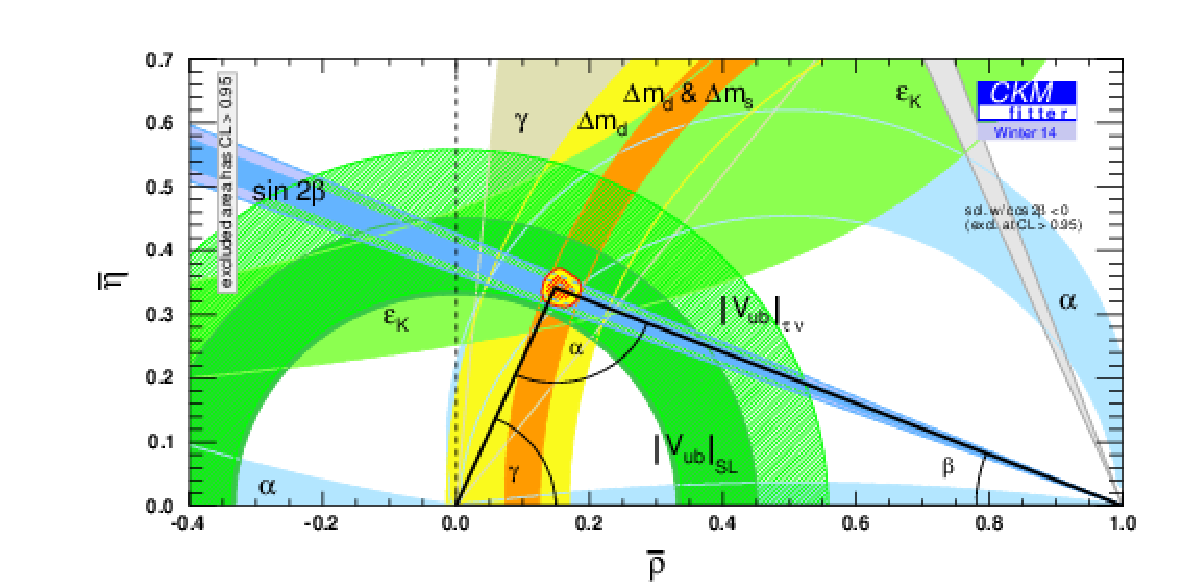
\includegraphics[width=0.80\textwidth]{rhoeta_small_Vub}
  \end{center}
  \caption[Unitarity triangle and current constraints]
  {
    Diagram of the \ut with coloured bands indicating various constraints on
    side lengths, angles and position of the apex, which is taken from the CKMfitter group in
    Ref.~\protect\cite{Charles:2015gya}.
    The constraints on \V{ub} from the combination of inclusive and exclusive modes
    ($\left|\V{ub}\right|_\mathrm{SL}$) is given separately to a value obtained using
    $\BF\left(\decay{\Bp}{\taup\nu_\tau}\right)$, ($\left|\V{ub}\right|_{\tau\nu}$).
  }
  \label{fig:th:ckmfitter}
\end{figure}

Unnatural \np models with parameters that differ wildly in magnitude tend to
lead to parameters or processes that must cancel to absurdly
high precision in order to agree with experimental observations.
These precise cancellations are known as \emph{fine tuning}.
In the \sm, quantum loop corrections to the Higgs mass are of the order $10^{19}$
for $m_H\simeq125\gev$~\cite{Chatrchyan:2012ufa,Aad:2012tfa}.
This means that the cancellations required to result in a Higgs mass comparable to the masses of
the weak vector bosons must be exact to 17 orders of magnitude.
This instance of fine tuning is known as the \emph{hierarchy problem}.
A solution for the hierarchy problem is to introduce \np particles, whose contributions to
loop level processes reduce the magnitude of fine tuning required to a level deemed
acceptable.
\SUSY immediately solves the hierarchy problem because for every \sm particle that
contributes to the Higgs mass, a \SUSY particle also contributes, but with the opposite sign.
It should be noted, however, that while \SUSY does solve a number of problems, it is not natural
since it has far more free parameters than the \sm.

Fine tuning also appears in \QCD.
A gauge invariant term that can be added to \Lag{QCD} is
\begin{equation}
  \Lag{QCD}^\theta = \theta\frac{g^2}{32\pi^2}
  G_{\mu\nu}^a\widetilde G^{\mu\nu}_a,
  \label{eq:strongcp}
\end{equation}
where $\theta$ and $g$ are constants.
The operator $G_{\mu\nu}$ is the gluon field strength tensor, and
\begin{equation}
  \widetilde G^{\mu\nu}_a = \frac12\varepsilon_{\mu\nu\rho\sigma}G^{\rho\sigma}_a.
\end{equation}
Interactions in $\Lag{QCD}^\theta$ would conserve \gls{C} symmetry, but violate both \gls{P} and
\gls{T} conjugation~\cite{Peccei:2006as}.
Such symmetry violations contradict the observed properties of the strong
force, so $\Lag{QCD}$ must either be absent, or heavily suppressed.
Bounds placed on the value of the neutron dipole moment, $|d_n| <2.9\e{-26}\,\mathrm{ecm}$
(at 90\% CL)~\cite{Baker:2006ts} leads to the constraint that
$\theta<10^{-19}$~\cite{Crewther:PQref9}, when \emph{a priori} it could be in the range
$0<\theta<2\pi$.
This occurrence of fine tuning is referred to as the \emph{strong \CP problem}.

Despite the evidence for \bsm physics and the list of problems that must be solved, its precise
manifestation is unknown.
There are numerous theories concerning NP scenarios which seek to solve various problems.

%Some models have a \emph{dark} or \emph{hidden} sector which, apart from gravity, only
%communicates with the visible sector feebly via messenger particles.
%These messenger particles could potentially be observed after they decay into \sm particles after
%mixing with a $H$, $Z$, $\gamma$ or $\nu$.
A solution to the strong \CP problem is to introduce an additional chiral $U(1)$ symmetry,
which is known as a \gls{PQ} symmetry~\cite{Peccei:2006as}.
Breaking the $U_\mathrm{PQ}(1)$ symmetry leads to $\theta$, in \Eq{eq:strongcp}, becoming a
field with quanta known as \emph{axions}.
These axions could be the messenger particle between a dark and visible
sector~\cite{Peccei:2006as}.

%%%%%%%%%%%%%%%%%%%%%%%%%%%%%%%%%%%%%%%%%%%%%%%%%%%%%%%%%%%%%%%%%%%%%%%%%%%%%%%%%%%%%%%%%%%%%%%%%%
%%%%%%%%%%%%%%%%%%%%%%%%%%%%%%%%%%%%%%%%%%%%%%%%%%%%%%%%%%%%%%%%%%%%%%%%%%%%%%%%%%%%%%%%%%%%%%%%%%
%%%%%%%%%%%%%%%%%%%%%%%%%%%%%%%%%%%%%%%%%%%%%%%%%%%%%%%%%%%%%%%%%%%%%%%%%%%%%%%%%%%%%%%%%%%%%%%%%%




%%%%%%%%%%%%%%%%%%%%%%%%%%%%%%%%%%%%%%%%%%%%%%%%%%%%%%%%%%%%%%%%%%%%%%%%%%%%%%%%%%%%%%%%%%%%%%%%%%
%%%%%%%%%%%%%%%%%%%%%%%%%%%%%%%%%%%%%%%%%%%%%%%%%%%%%%%%%%%%%%%%%%%%%%%%%%%%%%%%%%%%%%%%%%%%%%%%%%
%%%%%%%%%%%%%%%%%%%%%%%%%%%%%%%%%%%%%%%%%%%%%%%%%%%%%%%%%%%%%%%%%%%%%%%%%%%%%%%%%%%%%%%%%%%%%%%%%%


Some searches look directly for evidence of NP, this is the case for the analysis detailed in
\Chap{ch:db}, where a new particle, \db, is searched for in the dimuon invariant mass spectrum of
\decay{\Bd}{\Kstarent\mumu} consistent with \decay{\db}{\mumu}.
This is sensitive to a range of models which predict a light particle with a mass in the range
$2m_\mu\lesssim m_\db\lesssim4000\mev$, such as the axion model.
It is also sensitive to the $P^0$ that was hinted at by the Hyper-\CP
experiment~\cite{Park:2005eka}.

Instead of counting on NP to behave in an expected way, it is possible to search in a model
independent manner by exploring general physics couplings.
To do this it is useful to introduce the \OPE~\cite{PhysRev.179.1499}.


